\begin{ZhChapter}
    \chapter{Related Work}
    In the following section, we will introduce the concept of metaheuristics \cite{yang2010nature,yang2011metaheuristic} . Then, we will discuss the importance of loss functions and their role in deep learning \cite{deepLearning} models. Finally, we will explore image classification \cite{rawat2017deep} and its real-life applications.

    \section{Metaheuristic}
    Metaheuristic \cite{glover1986future} was first proposed by \citeauthor{glover1986future}. It can be regarded as a high-level procedure used to find solutions to optimization problems or other issues that conventional algorithms cannot solve. Within metaheuristics, an important concept is that these procedures must find a potentially optimal solution under reasonable computational costs or insufficient information. In this paper, we will primarily focus on nature-inspired metaheuristics \cite{yang2010nature}. In these methods, a common approach is to use a population-based strategy to find the optimal solution. Within a population, each individual typically represents a potential solution. We perform various operations on the individuals within the population to achieve our goal of approximating the optimal solution. A subset of specialized algorithms falls under population-based methods \cite{enwiki:1255593755}, commonly referred to as evolving algorithms (EAs) \cite{muhlenbein1988evolution}. Commonly used methods within EAs include genetic algorithms (GA) \cite{kumar2010genetic}, genetic programming (GP) \cite{geneticProgramming} , evolutionary programming (EP) \cite{yao1999evolutionary}, and differential evolution (DE) \cite{das2010differential}. We will briefly discuss EAs and GAs, and then we will focus primarily on GPs in the following paragraph.

    EAs can be described as algorithms inspired by the concept of "survival of the fittest \cite{paul1988selection}." These algorithms often take cues from natural evolutionary mechanisms to create algorithms that mimic animal behavior in the search for optimal solutions. Common examples include Ant Colony Optimization (ACO) \cite{dorigo2006ant}, GA, and Particle Swarm Optimization (PSO) \cite{kennedy1995particle}. In this type of algorithm, the typical approach is to initialize a population, which consists of several individuals. Each individual represents a potential optimal solution. After initializing the population, we usually set a number to represent how many generations we want this population to evolve. Before the start of each generation, a special function is used to calculate the fitness value of each individual, determining their level of excellence. Next, we perform selection, mutation, and crossover on the population. Selection involves choosing individuals based on their fitness to reproduce the next generation. Mutation generally refers to making random changes to an individual, while crossover combines the characteristics of two individuals to create the next generation. These steps are repeated until the predefined number of generations is reached, or the individuals fail to achieve the expected results, leading to a forced stop. Ultimately, the best individual in the population is obtained as the solution.

    GA is considered a type of EA, utilizing the representation of each solution in the form of chromosomes to perform selection, mutation, and crossover. GP is regarded as a special case of GAs, but due to its versatility and practicality, it is seen as a reliable solution. Unlike GAs, GP typically uses a more robust encoding method to represent chromosomes. For instance, GAs often use strings to represent chromosomes, which can present potential issues that need to be addressed, such as the priority of operations for each symbol or the validity of the equation itself. In contrast, GP usually represents chromosomes as trees, a method that can employ predefined traversal techniques to avoid these issues. It is worth noting that in GAs and GP, we can leverage their inherent ability to evolve automatically to find a reasonable optimal solution without having an in-depth understanding of the knowledge domain related to the problem we aim to solve. In the following paragraphs, we will introduce related research.

    In \cite{coreyes2022evolvingreinforcementlearningalgorithms}, \citeauthor{coreyes2022evolvingreinforcementlearningalgorithms} proposed a meta-learning reinforcement learning algorithm. They used computational graphs to represent algorithms. By doing so, algorithms could be identified, calculated, and optimized through Reinforcement Learning (RL) \cite{kaelbling1996reinforcement}. Notably, in this study, algorithms were represented as directed acyclic graphs (DAG) \cite{thost2021directedacyclicgraphneural} of nodes. Within the DAG , all nodes were classified into three categories: input nodes, parameter nodes, and operation nodes. Once the algorithms were represented as DAGs, they could be placed into RL for training and evaluation. In this proposed algorithm, they employed the concept of regularized evolution \cite{real2019regularized} to evolve a population formed by several randomized and known algorithms. The method was as follows: initialize the population with algorithms, evaluate each algorithm in the population and record their performance, then in a loop, repeatedly use a sample tournament \cite{goldberg1991comparative} to select algorithms, perform mutations on the algorithms by the mutator they designed, and evaluate them again until the loop ends. During the evaluation process, they trained and assessed the algorithms using RL, continuously testing the performance of each algorithm in different training environments. They also utilized normalized training performance to avoid numerical biases caused by varying environments. Through this approach, the study successfully created two algorithms, named DQNClipped and DQNReg, which outperformed classical control tasks.

    In \cite{akhmedova2024generationlossfunctionimage}, \citeauthor{akhmedova2024generationlossfunctionimage} proposed a genetic programming-based method to find a better function for the image classification training task. They encoded the loss functions into trees, with each tree considered an individual. All individuals were aggregated into a population. In this study, the population was evolved across multiple generations. Before the start of each generation, all individuals were evaluated. Each individual had a probability of undergoing crossover with an individual from a special external archive to create a new individual; otherwise, it would perform the crossover with another individual. Following this, two probabilistic decisions were made. If successful, the new individual could perform subtree mutation or one-point mutation, respectively. At the end of each generation, the fitness value of all individuals was re-evaluated. A certain number of low-scoring individuals were eliminated to the special external archive mentioned earlier, maintaining the stability of the population's size. After these steps, a new generation began, continuing until a predefined number of generations was reached.  By employing this method, this study successfully evolved an outstanding individual within the population, creating a function that could train an image classification model more effectively compared to Cross Entropy (CE) \cite{zhang2018generalized}.

    \section{Loss Function}

    \subsection{Deep Learning Model}
    In recent years, due to the significant increase in the computational speed of GPUs, training deep learning models to solve a wide variety of problems has become widely regarded as a feasible and popular solution. The process of training a deep learning model is often divided into several steps: collecting the data needed to train the model, and adding ground truth values to the data according to the model's requirements. Ground truth can be thought of as the ideal answers we hope to achieve after the model's computation. Once the data collection is complete, these data sets are collectively referred to as the dataset. Typically, the dataset is divided into training sets, validation sets, and testing sets. Data from the training set are used to train the model, the validation set is used to evaluate the model's effectiveness after each training loop, and the testing set is used to calculate the model's final score and determine whether the model successfully achieves its designed purpose. It is worth noting that the testing set data should not be seen during training and validation phases. After dividing the dataset, we decide on the model's architecture. Common architectures include Fully Connected Networks (FCN) \cite{iliadis2018deep} and Convolutional Neural Networks (CNN) \cite{wu2017introduction}, etc. Then the training process can begin. During training, we compare the model's output with the ground truth of the training data and use a loss function to calculate the difference between the output and the ground truth. This guides the adjustment of the model's parameters. Therefore, the loss function significantly determines the effectiveness of model training, and this aspect will be explained further later. After adjusting the model, the next round of training begins, continuing until the training is deemed ineffective or a predetermined maximum number of iterations is reached.
    \subsection{Importance of Loss Function}
    In \cite{gonzalez2020improvedtrainingspeedaccuracy}, a loss function meet genetic programming is proposed ....
    \section{Image Classification}

    % \subsection{}
    % 定義定義定義定義定義定義\cite{latex2e},定義定義定義定義,定義定義定義定義定義定義定義定義定義定義,定義定義。

    % \begin{table*}[htbp]
    %     \centering
    %     \caption{表格範例標題} \label{tab: complexity}
    %     \makebox[\linewidth][c]{
    %     \renewcommand\arraystretch{1.2}{
    %         \begin{tabular}{| l | c  c  c  c |}
    %         \hline
    %         Protocol & $P$ & $CS_1$ & $CS_2$ & $RG$ \\
    %         \hline
    %         MSSMul & $O(1)$, $O(1)$, N/A & $O(n-t)$, $O(n)$, $O(1)$ & $O(n-t)$, $O(n)$, N/A & $O(1)$, $O(n)$, $O(n)$ \\
    %         SC & $O(1)$, $O(1)$, N/A & $O(n-t)$, $O(n)$, $O(1)$ & $O(n-t)$, $O(n)$, N/A & $O(1)$, $O(n)$, $O(n)$ \\
    %         \hline 
    %         \end {tabular}
    %     }}
    % \end {table*}

    % \section{模型說明(小標)}

    % 說明說明說明說明,說明說明說明說明說明說明說明說明說明說明說明說明,說明說明說明說明說明說明說明說明。

    % \begin{figure*}[htbp]
    %     \centering
    %     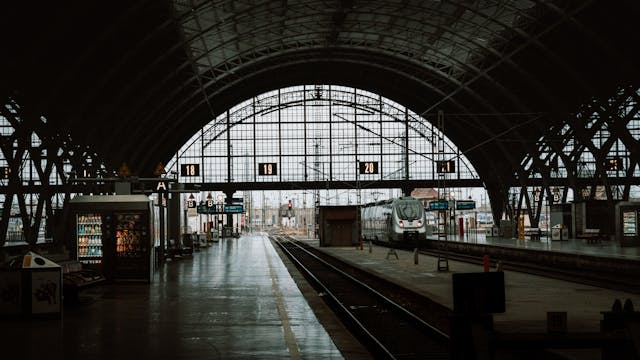
\includegraphics[width = 0.5\textwidth]{image.jpeg}
    %     \caption{Cool train station}
    %     \label{fig: image}
    % \end{figure*}

\end{ZhChapter}